\documentclass[12pt]{scrarticle}

\usepackage[english]{babel}    
\usepackage[T1]{fontenc}       
\usepackage[utf8]{inputenc} 
\usepackage{amsmath}           
\usepackage{amsfonts}          
\usepackage{amssymb}
\usepackage{amsthm}
\usepackage{graphicx} 
\usepackage{typearea}	        
\usepackage{scrlayer-scrpage}
\usepackage{lastpage}          
\usepackage{physics}
\usepackage{url}
\usepackage[margin=10pt,font=small,labelfont=bf]{caption}
\usepackage{subcaption}
\usepackage{comment}
\usepackage{hyperref}
\usepackage{siunitx}
\usepackage{placeins}
\usepackage{verbatim}
\usepackage{cleveref}
\usepackage{braket}
\usepackage{dsfont}
\usepackage{geometry}
\geometry{margin=1in}

\sisetup{separate-uncertainty, locale = UK}
\usepackage[backend=biber,sorting=none,style=numeric-comp]{biblatex}
\DeclareSIUnit\litre{l}

\addbibresource{ref.bib}

\newcommand{\dS}{\mathrm{dS}}
\newcommand{\phys}{\mathrm{phys}}


\title{Spacetime Density Kernel and the DSSYK Two-Point Function}
\author{Max, Georg}
\date{\today}

\begin{document}

\maketitle

\section{Setup: the Spacetime Density Kernel}

Given a Hilbert space $\mathcal{H}$ with density matrix $\rho$, time evolution $U_t = e^{-iHt}$,
and a bipartition $\mathcal{H} = \mathcal{H}_A \otimes \mathcal{H}_B$ with matrix unit bases
$\hat{E}^A_{ij} = \ketbra{i}{j} \otimes \mathbf{1}_B$ and
$\hat{E}^B_{kl} = \mathbf{1}_A \otimes \ketbra{k}{l}$,
the \emph{spacetime density kernel} (SDK) coefficients are defined by
\begin{equation}
    C_{ij;kl}(t) = \text{Tr}\!\left[\rho\,\hat{E}^A_{ij}\,U_t^\dagger\,\hat{E}^B_{kl}\,U_t\right].
    \label{eq:SDK_def}
\end{equation}
The SDK encodes two-time correlators via
\begin{equation}
    \mathcal{L}_t(O_A, O_B)
    \;=\; \text{Tr}\!\left[\rho\,O_A\,U_t^\dagger\,O_B\,U_t\right]
    \;=\; \sum_{i,j,k,l} C_{ij;kl}(t)\,O^{(A)}_{ij}\,O^{(B)}_{kl},
    \label{eq:correlator_from_SDK}
\end{equation}
where $O^{(A)}_{ij} = \bra{i}O_A\ket{j}$ and $O^{(B)}_{kl} = \bra{k}O_B\ket{l}$
are the matrix elements in the chosen basis.

\section{Single-Sided DSSYK}

\subsection{Energy basis and overlaps}

The single-sided DSSYK Hilbert space is spanned by chord number states $\ket{n}$,
$n = 0,1,2,\ldots\;$. To compute the SDK coefficients we initially take
$\rho = \ketbra{0}{0}$, the chord vacuum. As we will discuss later,
reproducing the NV two-point function requires instead the maximal entropy state
$\rho = \ketbra{E_0}{E_0}$.
The continuous energy eigenstates $\ket{\theta}$ satisfy the resolution of identity
\begin{equation}
    \mathbf{1} = \int_0^\pi \frac{d\theta}{2\pi}\,\mu(\theta)\,\ketbra{\theta}{\theta},
    \qquad
    \mu(\theta) = \{ q,\,e^{\pm 2i\theta}; q\}_\infty
    \label{eq:resolution}
\end{equation}
with the inner product 
\begin{equation}
    \braket{\theta|\phi} = \frac{2\pi\,\delta(\theta-\phi)}{\mu(\theta)}.
    \label{eq:inner_product}
\end{equation}
The overlaps with chord basis states are
\begin{equation}
    \braket{\theta|n} = \frac{H_n(\cos\theta| q)}{\sqrt{(q;q)_\infty}},
    \label{eq:overlap}
\end{equation}
where $H_n(x| q)$ are the continuous $q$-Hermite polynomials, $H_0 = 1$.
The energy is parametrized by
\begin{equation}
    E(\theta) = -\frac{2J\cos\theta}{\sqrt{\lambda(1-q)}}.
    \label{eq:dispersion}
\end{equation}

\subsection{SDK coefficients}

Inserting two resolutions of identity \eqref{eq:resolution} into \eqref{eq:SDK_def}
and using $\rho = \ketbra{0}{0}$ gives
\begin{align}
    C_{ij;kl}(t)
    &= \int\frac{d\theta\,d\phi}{(2\pi)^2}\,\mu(\theta)\mu(\phi)\,
       e^{-it(E(\theta)-E(\phi))}\,
       \bra{0}\hat{E}^A_{ij}\ket{\theta}\,
       \bra{\theta}\hat{E}^B_{kl}\ket{\phi}\,
       \braket{\phi|0}.
    \label{eq:SDK_inserted}
\end{align}
Evaluating each matrix element,
\begin{equation}
    \bra{0}\hat{E}^A_{ij}\ket{\theta}
    = \braket{0|i}\braket{j|\theta}
    = \delta_{0i}\,\frac{H_j(\cos\theta| q)}{\sqrt{(q;q)_\infty}},
\end{equation}
\begin{equation}
    \bra{\theta}\hat{E}^B_{kl}\ket{\phi}
    = \braket{\theta|k}\braket{l|\phi}
    = \frac{H_k(\cos\theta| q)\,H_l(\cos\phi| q)}{(q;q)_\infty},
\end{equation}
\begin{equation}
    \braket{\phi|0} = \frac{H_0(\cos\phi| q)}{\sqrt{(q;q)_\infty}} = \frac{1}{\sqrt{(q;q)_\infty}}.
\end{equation}
Substituting back into \eqref{eq:SDK_inserted} and absorbing overall factors of $(q;q)_\infty$
into a proportionality constant,
\begin{equation}
    \boxed{
    C_{ij;kl}(t) \propto \delta_{0i}
    \int\frac{d\theta\,d\phi}{(2\pi)^2}\,\mu(\theta)\mu(\phi)\,
    e^{-it(E(\theta)-E(\phi))}\,
    \frac{H_j(\cos\theta| q)^*}{\sqrt{(q;q)_j}}
    \frac{H_k(\cos\theta| q)}{\sqrt{(q;q)_k}}
    \frac{H_l(\cos\phi| q)}{\sqrt{(q;q)_l}}.
    }
    \label{eq:SDK_result}
\end{equation}

\subsection{Special case: SFF like Frobenius norm}
We can simplify the expression, if we calculate the $F_2$-norm from the kernel. The full kernel can be expressed as
\begin{align}
    C_{ij;kl}(t) = 
    \braket{0|\rho|i} \int \frac{d\theta d\phi}{(2\pi)^2} \ \mu(\theta) \mu(\phi) \
    e^{-i t(E(\theta)-E(\phi))} 
    \frac{H_j^*(\cos \theta |q) H_k(\cos \phi|q)}{\sqrt{(q;q)_j (q;q)_k}} \ 
    \frac{H_l^*(\cos\theta |q)}{\sqrt{(q;q)_l}}.
\end{align}
For the case of $\rho = \ketbra{0}{0}$ we can calculate the frobenius norm
\begin{align}
    \sum_{i,j} C_{ij;ji}(t) &= \sum_{i,j} \delta_{0i} \int \frac{d\theta d\phi}{(2\pi)^2} \ \mu(\theta) \mu(\phi) \
    e^{-i t(E(\theta)-E(\phi))} 
    \frac{\left| H_j(\cos{\phi}|q) \right|^2}{(q;q)_j} \ 
    \frac{H_i^*(\cos\theta |q)}{\sqrt{(q;q)_i}},
\\
    &= \int^\pi_0 \int^\pi_0 \frac{d\theta d\phi}{(2\pi)^2} \ \mu(\theta) \mu(\phi) \
    e^{-i t(E(\theta)-E(\phi))} 
    \label{eq:cijji}
\end{align}

This turns out to be just the square of the absoute value of one integral:
\begin{align}
     \sum_{i,j} C_{ij;ji}(t) = \left| \int_0^\pi \frac{d \theta}{2 \pi} \mu(\theta) e^{-itE(\theta)} \right|^2.
\end{align}
However, this just the integral over the absolute square of the well known DSSYK partition function, or to be more exact its analytically continuation. In \cite{berkooz_chord_2018} equation (4.10) the expression for the partition function is
\begin{align}
    Z(\beta) = \int_0^\pi d\phi e^\frac{2 \beta \cos(\phi)}{\sqrt{\lambda}} \Psi(\phi; q),
\end{align}
where $\Psi(\phi; q)$ matches our $\mu(\phi)/2\pi$. Also in chapter 4 of the paper the limit $q\rightarrow 1^-$ of this partition function is taken in detail.

\subsection{Numerical evaluation of the SFF like Frobenius norm}
The sum over $C_{ij;ji}$ was calculated numerically involving numerical integration in Mathematica of integral \cref{eq:cijji}. The integrand is highly oscillating especially for large $t$ and also for high $q$ values.
\begin{figure}[htbp]
    \centering
    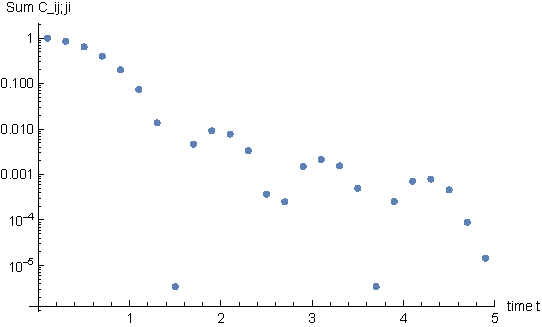
\includegraphics[width=0.5\linewidth]{plots/C_num.pdf}
    \caption{Numerical integration of expr. \cref{eq:cijji} for a value of $q = 0.1$}
    \label{fig:cijji_5}
\end{figure}

The computation (Mathematica) takes a long time due to higher oscillations for bigger $t$ and low $\lambda$, which is the regime we are interested in...
\begin{figure}[htbp]
    \centering
    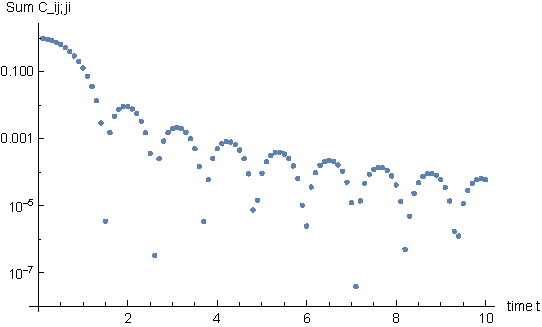
\includegraphics[width=0.5\linewidth]{plots/C_num2.pdf}
    \caption{Numerical integration of expr. \cref{eq:cijji} for a value of $q = 0.1$}
    \label{fig:cijji_50}
\end{figure}

\section{Calculating Two Time Correlators}
The purpose of defining a general response tensor $C_{ij;kl}$ is to easily compute two time correlators $\mathcal{L}_t(O_A, O_B)$ via the formula
\begin{align}
    \mathcal{L}_t(O_A, O_B) &= \text{Tr}\left[ \rho O_A U_t^\dagger O_B U_t \right] \nonumber \\
        &= \text{Tr}\left[T_{AB}(t) (O_A \otimes O_B) \right] \nonumber \\
        &= \sum_{i,j, k, l} C_{ij;kl} \ O_{ij}^{(A)} O_{kl}^{(B)}.
        \label{eq:two_time_c}
\end{align}
We briefly want to check that the kernel indeed does so by reproducing the two time correlator for the DSSYK given in \cite{berkooz_towards_2018} in eq. (3.16).

The observables in DSSYK are usually insertions of operators $M$ into our chord diagrams, which are simply fermion strings with random gaussian coefficients similar to the ones in our Hamiltonian. It is possible to compute the correlators via chord diagrams where each crossing of an $M$-string with an $H$-string is counted with a factor $\Tilde{q}$. In the analytic description one inserts a matrix 
\begin{align}
    S = \begin{pmatrix}
        1 & 0 & 0 & \ldots \\ 
        0 & \Tilde{q} & 0\\
        0 & 0&\Tilde{q}^2 \\
        \vdots & & & \ddots
    \end{pmatrix}.
\end{align}
So the operator coefficients we need are
\begin{align}
    O_{ij} = \delta_{ij} \ \Tilde{q}^j.
\end{align}

We use $\cos(\theta) = x$ and $\cos(\phi) = y$. With this and $\rho = \ketbra{0}{0}$ equation \cref{eq:two_time_c} reads
\begin{align}
    \sum_{i,j, k, l} C_{ij;kl} \ O_{ij}^{(A)} O_{kl}^{(B)} = \sum_{i,j,k,l} \int &\frac{d\theta d\phi}{4 \pi^2} \mu(\theta) \mu(\phi) e^{i t(E(\theta) - E(\phi))} \cdot \nonumber
    \\ &\frac{H_j(x|q)}{\sqrt{(q;q)_j}} \frac{H_k(y|q) H_l(x|q)}{\sqrt{(q;q)_k}\sqrt{(q;q)_l}} \delta_{0i} \delta_{ij} \Tilde{q}^i \delta_{kl} \Tilde{q}^k
\end{align}
which simplifies to
\begin{align}
    \sum_{i,j, k, l} C_{ij;kl} \ O_{ij}^{(A)} O_{kl}^{(B)} 
    = \sum_{k} \int \frac{d\theta d\phi}{4 \pi^2} \mu(\theta) \mu(\phi) e^{i t(E(\theta) - E(\phi))} \frac{H_k(y|q) H_k(x|q)}{(q;q)_k} \Tilde{q}^k.
 \end{align}
Now we can use the identity for q-Hermite polynomials from \cite{berkooz_towards_2018} eq. (B.12) in the form \cref{eq:generating_funct} to get the desired form
\begin{align}
     \sum_{i,j, k, l} C_{ij;kl} \ O_{ij}^{(A)} O_{kl}^{(B)} =
     \int \frac{d\theta d\phi}{4 \pi^2} \mu(\theta) \mu(\phi) e^{i t(E(\theta) - E(\phi))} \frac{(\Tilde{q}^2, q)_\infty}{(\Tilde{q} e^{i(\pm \theta \pm \phi)}; q)_\infty},
\end{align}
which we can find in \cite{berkooz_towards_2018} eq. (3.16) for euclidean time evolution.

\section{Doubled SYK model}
In the following, we want to calculate the coefficients $C_{ij;kl}$ of the spacetime density kernel $T_{AB}$ for the doubled SYK model of Narovlansky and Verlinde \cite{Narovlansky2023}. We consider a bipartition of the system in the left and right SYK model. The starting point is, again, the formula
\begin{align}
    C_{ij; kl}(t) = \text{Tr} \left[ \rho \ \hat{E}_{ij}^L \ U_t^\dagger \ \hat{E}_{kl}^R \ U_t \right]
\end{align}
Here, $i$ and $j$ are chord numbers in the left subsystem, while $k$ and $l$ are chord numbers in the right subsystem. As shown by NV, the energy eigenstates of the system are given as paired eigenstates $\ket{E}=\ket{E}_L\ket{E}_R$. We insert two complete sets of energy eigenstates, labeled by $\theta$ and $\phi$, and obtain:
\begin{align}
    C_{ij;kl}(t) &= 
    \int \frac{d\theta d\phi}{(2\pi)^2} \ \mu(\theta) \mu(\phi) \bra{0}\rho \hat{E}_{ij}^L\ket{\theta} \bra{\theta}U_t^\dagger\hat{E}_{kl}^RU_t\ket{\phi}\braket{\phi|0}\\
    &= 
    \int \frac{d\theta d\phi}{(2\pi)^2} \ \mu(\theta) \mu(\phi) e^{-i t(E(\theta)-E(\phi))}\bra{0}\rho \hat{E}_{ij}^L\ket{\theta} \bra{\theta}\hat{E}_{kl}^R\ket{\phi}\braket{\phi|0}
\end{align}
The last scalar product simply yields 1. We evaluate the two matrix elements in this equation separately below. Firstly, we obtain, by setting $\rho=\ketbra{0}{0}$ for the density matrix:
\begin{align}
    \bra{0}\rho \hat{E}_{ij}^L\ket{\theta}&=(\bra{0}\otimes\bra{0})(\ketbra{i}{j} \otimes  \mathds{1}_R)(\ket{\theta}\otimes\ket{\theta})\\
    &=\braket{0|i}\braket{j|\theta}\braket{0|\theta}.
\end{align}
Secondly, we obtain 
\begin{align}
    \bra{\theta}\hat{E}_{kl}^R\ket{\phi}&=(\bra{\theta}\otimes\bra{\theta})( \mathds{1}_L\otimes \ketbra{k}{l})(\ket{\phi}\otimes\ket{\phi})\\
    &=\braket{\theta|\phi}\braket{\theta|k}\braket{l|\phi}.
\end{align}
Substituting back, we obtain:
\begin{align}
    C_{ij;kl}(t) &= \int \frac{d\theta d\phi}{(2\pi)^2} \ \mu(\theta) \mu(\phi) e^{-i t(E(\theta)+E(\phi))}\braket{0|i}\braket{j|\theta}\braket{0|\theta}\braket{\theta|\phi}\braket{\theta|k}\braket{l|\phi}\\
    &\propto\int \frac{d\theta d\phi}{(2\pi)^2} \ \mu(\theta) \mu(\phi) e^{-i t(E(\theta)+E(\phi))}\delta_{0i}\frac{H_j(\cos(\theta)|q)^*}{\sqrt{(q; q)_j}}\delta(\theta-\phi)\\
    &\quad\frac{H_k(\cos(\theta)|q)}{\sqrt{(q; q)_k}}\frac{H_l(\cos(\phi)|q)}{\sqrt{(q; q)_l}}\\
    &=\delta_{0i}\int \frac{d\theta}{2\pi}\mu(\theta)^2e^{-2i tE(\theta)}\frac{H_j(\cos(\theta)|q)^*}{\sqrt{(q; q)_j}}\frac{H_k(\cos(\theta)|q)}{\sqrt{(q;q)_k}} \frac{H_l(\cos(\theta)|q)}{\sqrt{(q; q)_l}}
\end{align}
We find that the result for $C_{ij;kl}(t)$ is given by a single integral. We would like to find a relation to the two-point function given by Verlinde, which we explore in the following section.


\section{Contraction with the Matter Operator}

\subsection{The operator and its matrix elements}

The physical matter operator $\mathcal{O}_\Delta$ in DSSYK is diagonal in the chord basis:
\begin{equation}
    O_{ij} = \bra{i}\mathcal{O}_\Delta\ket{j} = \delta_{ij}\,\tilde{q}^{\,i},
    \qquad \tilde{q} = q^\Delta.
    \label{eq:operator}
\end{equation}
In the chord diagram language, each crossing of an $M$-string with an $H$-string
contributes a factor $\tilde{q}$, so $\mathcal{O}_\Delta$ is represented by the
diagonal matrix $S = \mathrm{diag}(1,\tilde{q},\tilde{q}^2,\ldots)$.

The NV physical operator is a product of left and right local operators,
\begin{equation}
    \mathcal{O}^\phys_\Delta(\tau) = \int dt\,\mathcal{O}^L_{1-\Delta}(t)\,\mathcal{O}^R_\Delta(-t+\tau),
\end{equation}
so the full contraction requires \emph{two} operator coefficient matrices:
$O^L_{ij} = \delta_{ij}(\tilde{q}')^i$ with $\tilde{q}' = q^{1-\Delta}$, and
$O^R_{kl} = \delta_{kl}\tilde{q}^k$ with $\tilde{q} = q^\Delta$.

\subsection{Applying the Poisson kernel identity}

Contracting \eqref{eq:SDK_result} with $O^L_{ij}O^R_{kl}$ and using $\delta_{ij}$,
$\delta_{0i}$, $\delta_{kl}$, the $i=j=0$ constraint gives $(\tilde{q}')^0=1$,
and the sum over $k=l$ remains:
\begin{align}
    \mathcal{L}_\tau(\mathcal{O}^\phys_\Delta, \mathcal{O}^\phys_\Delta)
    \propto
    &\int\frac{d\theta\,d\phi}{(2\pi)^2}\,\mu(\theta)\mu(\phi)\,
    e^{-\tau(E(\theta)-E(\phi))}\,
    \left(\sum_j \frac{H_j(\cos\theta| q)\,H_j(\cos\phi| q)}{(q;q)_j}(\tilde{q}')^j\right)\times \nonumber\\
    &\times\left(\sum_k \frac{H_k(\cos\theta| q)\,H_k(\cos\phi| q)}{(q;q)_k}\tilde{q}^k\right).
    \label{eq:double_sum}
\end{align}
Each sum is evaluated using the Poisson kernel for
the continuous $q$-Hermite polynomials \cite{berkooz_towards_2018},
\begin{equation}
    \sum_{k=0}^\infty \frac{H_k(\cos\theta| q)\,H_k(\cos\phi| q)}{(q;q)_k}\,t^k
    = \frac{(t^2;q)_\infty}{(t\,e^{i(\pm\theta\pm\phi)};q)_\infty},
    \label{eq:Poisson_kernel}
\end{equation}
where the right-hand side is shorthand for the product over all four sign choices,
\begin{equation}
    (t\,e^{i(\pm\theta\pm\phi)};q)_\infty
    = (t\,e^{i(\theta+\phi)};q)_\infty\,(t\,e^{i(\theta-\phi)};q)_\infty\,
      (t\,e^{-i(\theta-\phi)};q)_\infty\,(t\,e^{-i(\theta+\phi)};q)_\infty.
\end{equation}
Here $t$ is the generating parameter; the left side is a formal power series in $t$
whose coefficients are the products $H_k(\cos\theta| q)H_k(\cos\phi| q)/(q;q)_k$.
In our context $t = \tilde{q} = q^\Delta$ encodes the scaling dimension of the operator.

Applying \eqref{eq:Poisson_kernel} to both sums in \eqref{eq:double_sum} with
$t=\tilde{q}=q^\Delta$ and $t'=\tilde{q}'=q^{1-\Delta}$ respectively,
\begin{equation}
    \mathcal{L}_\tau
    \propto
    \int\frac{d\theta\,d\phi}{(2\pi)^2}\,\mu(\theta)\mu(\phi)\,
    e^{-\tau(E(\theta)-E(\phi))}\,
    \frac{((\tilde{q}')^2;q)_\infty}{(\tilde{q}'\,e^{i(\pm\theta\pm\phi)};q)_\infty}
    \cdot
    \frac{(\tilde{q}^2;q)_\infty}{(\tilde{q}\,e^{i(\pm\theta\pm\phi)};q)_\infty}.
    \label{eq:after_identity}
\end{equation}

\subsection{Converting to $q$-Gamma functions}

Using the definition of the $q$-Gamma function,
\begin{equation}
    \Gamma_q(x) = (1-q)^{1-x}\frac{(q;q)_\infty}{(q^x;q)_\infty},
\end{equation}
and identifying $q^{is} = e^{i\theta}$, each $q$-Pochhammer factor converts as
\begin{equation}
    \frac{1}{(\tilde{q}\,e^{i(\pm\theta\pm\phi)};q)_\infty}
    = \frac{1}{\prod_{\epsilon_1,\epsilon_2=\pm}(q^{\Delta+i\epsilon_1 s_1+i\epsilon_2 s_0};q)_\infty}
    \propto \Gamma_q(\Delta \pm is_0 \pm is_1),
    \label{eq:pochhammer_to_gamma}
\end{equation}
and analogously for the $1-\Delta$ factor. The numerator factors give
$(\tilde{q}^2;q)_\infty = (q^{2\Delta};q)_\infty \propto 1/\Gamma_q(2\Delta)$, and
$((\tilde{q}')^2;q)_\infty \propto 1/\Gamma_q(2-2\Delta)$.

The Askey-Wilson measure converts as
\begin{equation}
    \mu(\theta) = \{q,\,e^{\pm 2i\theta}; q\}_\infty \propto \frac{(q;q)_\infty^3}{\Gamma_q(\pm 2is_1)}.
\end{equation}

\subsection{Collapsing the $\phi$ integral via the choice of $\rho$}
To match the NV correlator, we must replace $\rho = \ketbra{0}{0}$ by
\begin{equation}
    \rho = \ketbra{E_0}{E_0}, \qquad \ket{E_0} = \ket{\theta_0},
    \label{eq:rho_E0}
\end{equation}
where $\ket{E_0} = \ket{\Psi_\dS}$ is the maximal entropy state, an energy eigenstate
with spectral parameter $s_0$ and $E_0 = 0$. Since $\ket{E_0}$ is an energy eigenstate,
the overlap with the chord basis is
\begin{equation}
    \braket{E_0|n}
    = \braket{\theta_0|n}
    = \frac{H_n(\cos\theta_0\mid q)}{\sqrt{(q;q)_\infty}},
\end{equation}
and in particular $\braket{E_0|0} = 1/\sqrt{(q;q)_\infty}$, which is no longer
$\delta_{0i}$. Crucially, with $\rho = \ketbra{E_0}{E_0}$ the SDK integral
\eqref{eq:SDK_inserted} becomes
\begin{align}
    C_{ij;kl}(t)
    &= \int\frac{d\theta\,d\phi}{(2\pi)^2}\,\mu(\theta)\mu(\phi)\,
       e^{-it(E(\theta)-E(\phi))}\,
       \bra{E_0}\hat{E}^A_{ij}\ket{\theta}\,
       \bra{\theta}\hat{E}^B_{kl}\ket{\phi}\,
       \braket{\phi|E_0}.
\end{align}
Now $\braket{\phi|E_0} = \braket{\phi|\theta_0} = 2\pi\delta(\phi-\theta_0)/\mu(\phi)$
by the inner product \eqref{eq:inner_product}. The $\delta(\phi-\theta_0)$ collapses
the $\phi$ integral immediately, with the $1/\mu(\phi)$ canceling one power of $\mu(\phi)$
from the measure, leaving a single integral over $\theta$:
\begin{equation}
    C_{ij;kl}(t)\big|_{\rho=\ketbra{E_0}{E_0}}
    \propto
    \int\frac{d\theta}{2\pi}\,\mu(\theta)\,
    e^{-it(E(\theta)-E(\theta_0))}\,
    \bra{E_0}\hat{E}^A_{ij}\ket{\theta}\,
    \bra{\theta}\hat{E}^B_{kl}\ket{\theta_0}.
\end{equation}
The phase $e^{+itE(\theta_0)}$ is a constant overall factor (since $s_0$ is fixed)
and can be absorbed into normalization. The contraction with operator coefficients
then proceeds exactly as in Section~5.2--5.3, with $\phi$ replaced everywhere by
the fixed value $\theta_0$. Both applications of the Poisson kernel \eqref{eq:Poisson_kernel}
now involve arguments $(\cos\theta, \cos\theta_0)$ rather than $(\cos\theta, \cos\phi)$,
and the result is the single integral
\begin{equation}
    \boxed{
    \mathcal{L}_\tau(\mathcal{O}^\phys_\Delta, \mathcal{O}^\phys_\Delta)
    \propto
    \int_0^\pi \frac{d\theta}{2\pi}\,\mu(\theta)\,e^{-\tau E(\theta)}\,
    \frac{\Gamma_q(\Delta\pm is_0\pm is_1)\,\Gamma_q(1-\Delta\pm is_0\pm is_1)}
         {\Gamma_q(\pm 2is_1)\,\Gamma_q(2\Delta)\,\Gamma_q(2-2\Delta)},
    }
    \label{eq:final_correlator}
\end{equation}
where $s_1$ is the spectral parameter corresponding to $\theta$, and $s_0$ is the
fixed spectral parameter of the external state $\ket{E_0}$.

\section{Comparison with the NV Two-Point Function}

Equation~\eqref{eq:final_correlator} is precisely the DSSYK two-point function
of Narovlansky and Verlinde \cite{Narovlansky2023} (eq.~(11) of \cite{Verlinde2024}):
\begin{equation}
    G_\Delta(\tau_1)
    = \bra{E_0}\mathcal{O}_\Delta(\tau)\mathcal{O}_\Delta(0)\ket{E_0}
    = \int ds_1\,e^{-\tau_1 E(s_1)}\,
      \frac{\Gamma_q(\Delta\pm is_0\pm is_1)\,\Gamma_q(1-\Delta\pm is_0\pm is_1)}
           {\Gamma_q(\pm 2is_1)\,\Gamma_q(2\Delta)\,\Gamma_q(2-2\Delta)}.
    \label{eq:NV_correlator}
\end{equation}

Using the identity (eq.~(12) of \cite{Verlinde2024})
\begin{equation}
    \Gamma_q(x)\,\Gamma_q(1-x)
    = iq^{1/8}(1-q)(q;q)^3_\infty\,\frac{q^{x/2}}{\vartheta_1\!\left(\tfrac{i\lambda}{2\pi}x,\,q\right)},
    \label{eq:Gamma_theta_identity}
\end{equation}
each pair $\Gamma_q(\Delta\pm is_0\pm is_1)\,\Gamma_q(1-\Delta\pm is_0\pm is_1)$
in \eqref{eq:NV_correlator} can be rewritten in terms of Jacobi theta functions.
The spectral density becomes a single theta function,
\begin{equation}
    \rho(s) = \frac{1}{\Gamma_q(\pm 2is)} \propto \vartheta_1\!\left(\tfrac{\lambda}{\pi}s,\,q\right),
\end{equation}
and the full two-point function takes the form
\begin{equation}
    G_\Delta(\tau_1)
    = \int dE(s_1)\,e^{-\tau_1 E(s_1)}\,
      \frac{\vartheta_1\!\left(\tfrac{i\lambda}{\pi}\Delta,\,q\right)
            \prod_a \vartheta_1\!\left(\tfrac{\lambda}{\pi}s_a,\,q\right)}
           {\prod_a \vartheta_1\!\left(\tfrac{\lambda}{2\pi}(i\Delta\pm s_0\pm s_1),\,q\right)},
    \label{eq:theta_form}
\end{equation}
with $a\in\{0,1\}$. The equivalence between \eqref{eq:NV_correlator} and \eqref{eq:theta_form}
follows from the Jacobi triple product identity, which relates each $q$-Pochhammer factor
$(e^{2i\theta};q)_\infty$ to $\vartheta_1(\theta/\pi,q)$.


\section*{Appendix}

\begin{align}
    \sum_{k=0}^{\infty} H_k(x|q) H_k(y|q) \frac{t^k}{(q;q)_k} = \frac{(t^2; q)_\infty}{(t e^{i(\pm \theta \pm \phi)}; q)_\infty}
    \label{eq:generating_funct}
\end{align}

\newpage
\printbibliography

\end{document}
